\chapter{Aspekte eines Anmeldesystemes und Biometrie}
\strahlhofer

\section{Prozesse eines Anmeldevorgangs}
\begin{center}
\begin{figure}[h]
    \centering
    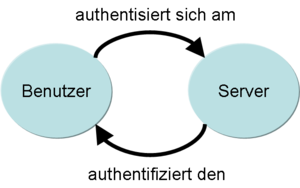
\includegraphics[width=9cm]{authentisieren-authentifizieren.png}
    \caption{Ablauf eines Anmeldevorgangs}
\end{figure}
\end{center}

%https://www.dr-datenschutz.de/authentisierung-authentifizierung-und-autorisierung/
\subsection{Authentisierung}
Bei der Authentisierung muss von einer Person ein Nachweis gegeben werden, dass sie die Person ist die sie behauptet zu sein. Dieser Nachweis kann durch drei verschiedene Methoden nachgewiesen werden, diese sind:
\begin{itemize}
	\item Die Person besitzt Wissen über eine Information, die nur der Kontoinhaber wissen kann, z.B. das Passwort oder Sicherheitsfragen sein.
	\item Das Individuum das sich versucht anzumelden und sendet beispielsweise einen Reisepass oder Führerschein als Konformation.
	\item Es wird vom Nutzer eine Information mitgesendet die er oder sie nur von sich selbst senden kann. Ein Beispiel wäre die Sendung von einem biometrischen Nachweis, dass kann entweder ein Fingerabdruck oder ein Gesichtsscan sein.
\end{itemize}

%https://www.dr-datenschutz.de/authentisierung-authentifizierung-und-autorisierung/
\subsection{Authentifizierung}
Bei diesem Schritt des Anmeldeablaufs, wird eine Überprüfung durchgeführt. Diese Prüfung soll analysiert die Informationen, die bei der Authentisierung erfasst worden sind. Können diese dem Zielkonto zugewiesen werden, dann ist der Nutzer die Person die er angibt zu sein.

%https://www.dr-datenschutz.de/authentisierung-authentifizierung-und-autorisierung/
\subsection{Autorisierung}
Die Autorisierung hat als Funktionalität die Bestätigung von bestimmten Rechten und Rollen zu bestimmten Ressourcen. Dieses Thema gehört der Informationssicherheit an und befasst sich mit der Zugriffskontrolle. Bei der Autorisierung wird für das Unternehmen ein Zugriffsmechanismus implementiert. Wenn z.B. ein Promoter sich in einem von der Firma erstellten System anmeldet, werden bestimmte Rollen und Rechte zugewiesen. Dies bedeutet das der Mitarbeiter nur einen bestimmten Zugriff auf gewisse Funktionalität besitzt.

\subsubsection{Rollen}
Bei der Anmeldung in die EMS-Software soll zwischen den Rollen Promoter und Administrator unterschieden werden. 
\begin{itemize}
	\item \textbf{Administratoren:} Die Rolle ist eine der wichtigsten in der Software. Dieser kann Benutzer und Events in einem System erstellen, verändern und löschen. Benutzer können zusätzlich deaktiviert werden, da diese entweder zu häufig falsche Anmeldeinformationen eingegeben haben oder weil die Person eine Anfrage darauf gestellt hat.
	\item \textbf{Promoter:} Diese Rolle sind Benutzer der Software, die Karten anfordern und verkaufen können. Sie können, beispielsweise die Funktionalitäten wie die Benutzer- und Eventverwaltung nicht bedienen.
\end{itemize}

%https://www.kaspersky.de/resource-center/definitions/biometrics
%Biometrie
\section{Biometrie}
%https://en.wikipedia.org/wiki/Biometrics
\subsection{Definition}
\begin{center}
	\textit{Biometrics are body measurements and calculations related to human characteristics}
\end{center}

Wie schon beschrieben ist, schließt eine biometrische Identifikation nur auf eine bestimmte Person zurück.
Durch diesen Aspekt ist die Biometrie eine sehr angesehne Identikationstechnik.
Eine biometrische Information kann durch viele unterschiedliche Methoden erhoben werden.
Folgende Charakterisiken können und werden heutzutage in vielen verschiedenen Arbeitsbereichen verwendet.
\begin{itemize}
	%https://www.livescience.com/62690-how-dna-ancestry-23andme-tests-work.html
	%https://www.ibia.org/biometrics-and-identity/biometric-technologies/dna#:~:text=DNA%20Biometrics,often%20in%20forensics%20and%20healthcare.&text=A%20feature%20of%20DNA%20identification,familial%20relationships%20via%20DNA%20testing.
	\item \textbf{DNA-Tests:} Ein DNA-Test wird in den unterschiedlichsten Arbeitsbereichen verwendet, z.B. in der Fornesik oder von der Polizei.
	Vorteile die DNA als biometrisches Mittel zu erwägen:
	\begin{itemize}
		\item Mit der DNA kann von einer unbekannten Person auf dessen Verwandten schließen. Dies ist die einzige biometrische Methode die diese Möglichkeit bietet.
		\item 
	\end{itemize}
	\item 
\end{itemize}



%iOS - Touchid
%Android - Fingerprint
%Sicherheit
%Genauigkeit
%Kosten
%Akzeptanz